%!TEX root = ../Main.tex

\chapter{Vulkan Rendering}
\label{cha:RenderPipeline}
  \todo[inline, color=blue!60]{Rename chapter? Current name matches with the names of the previous chapters but may be too general.}
  \todo[inline]{Image tiling and layout?}
  \todo[inline]{Resource transformations?}

  This chapter provides an overview of the steps required to render an image using the Vulkan graphics \gls{api}.
  Because there are many ways to perform rendering with Vulkan, a framework is defined that constrains the actual work that needs to be done to a comprehensible amount.

  First, the aforementioned framework is defined.
  Subsequently, the necessary Vulkan \gls{api} calls are shown and explained that are used to prepare for rendering.
  Following these preparations, recording of the actual rendering commands is presented.
  And finally, in the render loop, shader data is updated and rendering commands are submitted to the \gls{gpu}.
  Section~\ref{sec:MultithreadedRendering} at the end of this chapter provides additional information about multi-threaded rendering in Vulkan.

  Throughout this chapter, listings are presented that show the usage of select Vulkan commands and data structures that are required for rendering.
  It must be noted, however, that these listings are simplified in order to improve legibility.
  Tasks that need to be performed, such as memory allocation, may be shown in an abridged form.

  \section{Framework}
  \label{sec:Framework}
    A simple forward renderer is assumed which means that rendering is performed in a way that produces the presentable image in a single step.
    A camera is used to observe the scene.
    This camera is not fixed which means it may change position or rotation over time, changing how the scene is portrayed.
    The rendered scene will contain a fixed number of objects.
    Each object has fixed geometry and is assigned a position in an application-defined coordinate space.
    The shaders used to render each object are kept very simple.
    Objects do not have textures or other color information and are rendered in a solid color.
    Lighting is restricted to only produce flat shaded surfaces.
    The actual layout of these shaders is shown in section~\ref{subsec:GraphicsPipelineSetup}.

  \begin{figure}
    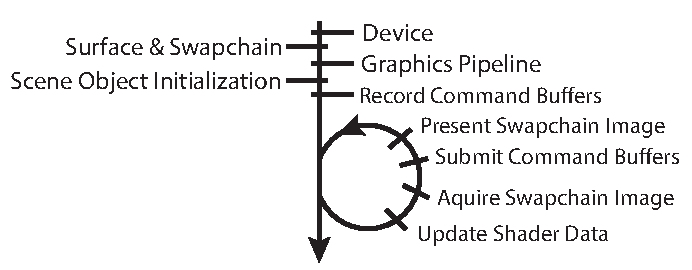
\includegraphics{Main/Images/RenderSetupAndLoopSimple}
    \centering
    \caption{Overview of the setup and execution of a simple forward-renderer in Vulkan as implemented in chapter~\ref{cha:RenderPipeline}.}
    \label{fig:RenderSetupAndLoopSimple}
  \end{figure}

  Figure~\ref{fig:RenderSetupAndLoopSimple} provides an abstract overview of this framework.
  The different steps depicted are explained in the course of this chapter.


  \section{Setup}
  \label{sec:RenderingSetup}
    Before an image can be rendered, proper Vulkan facilities need to be set up.
    Most of these facilities have been presented in chapter~\ref{cha:VulkanOverview}.
    In the following sections, these facilities are set up in the context of the framework defined in section~\ref{sec:Framework}.

    \subsection{Device and Queue Setup}
      The Vulkan device to be used for rendering needs to support both the swapchain extension as well as queues with graphics and present capabilities.

      In order for a rendered image to be presented to a window, the swapchain extension\footnote{Full name: \lstinline{VK_KHR_swapchain}} needs to be activated.
      This can be done when creating the device.
      Without this extension, no swapchain can be created for this device, which is necessary to present a rendered image in Vulkan.
      Note, however, that the swapchain is not automatically created at this point.
      This has to be done explicitly by the application and is explained later.

      \lstinputlisting[
        label=lst:FindQueueFamilyIndex,
        caption={Finding a queue family index with both graphics and present capabilities.},
        style=MyCppFloat,
        firstline=1,
        lastline=8,
        float
      ]
      {Main/Listings/CreateDeviceAndQueue.cpp}

      In Vulkan, rendering commands are submitted to a device queue.
      For the purposes of this chapter, queues with two specific capabilities are required.
      These capabilities are called the \textit{graphics capability} and the \textit{present capability}.
      The first specifies whether the queue supports graphics commands such as \lstinline{vkCmdDraw}.
      The second capability specifies whether \lstinline{vkQueuePresentKHR} is supported on that queue.
      Without both of these capabilities, rendering and presenting an image is not possible.
      A queue might support both of these capabilities but it is also possible that two separate queues are used for graphics and presenting, respectively.
      In this chapter, a single queue with both capabilities is assumed.

      \lstinputlisting[
        label=lst:DefineQueueCreateInfo,
        caption={Definition of a queue create info.},
        style=MyCppFloat,
        firstline=10,
        lastline=14,
        float
      ]
      {Main/Listings/CreateDeviceAndQueue.cpp}

      Once a queue with both capabilities has been found, information about an instance of this queue is defined as shown in listing~\ref{lst:DefineQueueCreateInfo}.
      The index of that queue is used on line~2 to specify which queue to create an instance from.
      This index will be used throughout this chapter for other kinds of operations.
      On line~4, the priority of this queue instance is set.
      Because only a single queue is used in this case, the priority is set to the highest value.
      Queues are not created explicitly by the application.
      Instead, queues are created along with the device they belong to.

      \lstinputlisting[
        label=lst:DeviceCreation,
        caption={Creation of a device with the swapchain extension as well as the retrieval of a queue from that device.},
        style=MyCppFloat,
        firstline=16,
        lastline=25,
        float
      ]
      {Main/Listings/CreateDeviceAndQueue.cpp}

      Listing~\ref{lst:DeviceCreation} shows the creation of the logical device that will be used for all subsequent Vulkan operations.
      On lines~1~and~6, the swapchain extension is requested for this device.
      On line~4, the queue create info is passed.
      And finally on line~8, the logical device and the queue are created.
      Line~10 shows how the queue is retrieved from the created device.
      This queue will be used to submit rendering commands to the \gls{gpu} and for interaction with the presentation engine.

    \subsection{Creating a Surface and a Swapchain}
      Now that a device with the enabled swapchain extension is in place, a swapchain can actually be created.
      Creating a swapchain requires what is called a Vulkan \textit{surface} to be created first.
      This surface is specific to the operating system and represents the connection to the actual window.
      It is also the target of the presentation engine which means that this surface is used to present a rendered image.

      \todo[inline]{Number, format, extent, colorspace of swapchain images.}
      \todo[inline]{Present modes / VSync.}
      A swapchain consists of multiple images.
      These images are managed by the presentation engine.
      The application may require the swapchain to create a certain number of images constrained to a range defined by the surface.

      The exact settings of a swapchain or a surface are not relevant for the purposes of this chapter.
      Because of that, no listings about the details of creating these objects are presented.

      The reason why an application may care about the number of swapchain images is rather straight-forward.
      From the point of view of the presentation engine, a swapchain image passes several stages until it is presented eventually.
      Initially the image is free and can be acquired by the application.
      Once an application acquires the image it is considered to be in use by the application and no longer free.
      At some point, the application hands back the image to the presentation engine, requesting that image to be presented.
      In the \gls{fifo} presentation mode, the image will be put into a queue to be processed by the presentation engine at a convenient time\todo{Explain more presentation modes?}.
      Once that time has come, the image will actually be presented on the surface.
      While an image is either currently presented or still pending presentation in the queue, it cannot be acquired by the application for rendering.
      When there is no free swapchain image, and the application tries to acquire one, the application will be stalled until a swapchain image is available.
      Depending on the chosen presentation mode, the number of swapchain images can be tuned to find the balance that works best for the application.
      Using too many swapchain images wastes memory but not having enough images may stall the application.

      Swapchain images will be used exclusively as color attachments for the framebuffer in this chapter.

    \subsection{Preparing the Graphics Pipeline}
    \label{subsec:GraphicsPipelineSetup}
      The graphics pipeline controls how data is processed on the \gls{gpu}.
      It has many components that need to be initialized.
      The process of preparing for the creation of a graphics pipeline is demonstrated in the following sections.
      Furthermore, the creation of an actual graphics pipeline object is shown in section~\ref{sub:ActualGraphicsPipelineCreation}.

      \subsubsection{Shader Stages}
      \label{sss:GraphicsPipelineShaderStages}
        Among other things, the graphics pipeline consists of multiple shader stages.
        For each shader stage, the application needs to supply the actual shader code in \gls{spirv} format, as mention in previous chapters.
        For the purposes of this chapter, only a vertex shader and fragment shader will be used.

        \lstinputlisting[
          label=lst:ShaderStageSetup,
          caption={Setup of the shader stages for chapter~\ref{cha:RenderPipeline}.},
          style=MyCppFloat,
          firstline=4,
          lastline=10,
          float
        ]
        {Main/Listings/GraphicsPipelineSetup.cpp}

        Listing~\ref{lst:ShaderStageSetup} shows how information about the shader stages is specified.
        This information will be supplied to the graphics pipeline later.
        The types of the used shader stages is set on line~2 for the vertex shader and on line~5 for the fragment shader.
        Both shaders are loaded from a file on lines~3~and~6, respectively.
        As specified by the framework in section~\ref{sec:Framework}, shaders are kept very simple.
        The contents of these shaders are examined below.

        \lstinputlisting[
          label=lst:VertexShader,
          caption={Simplified vertex shader used in chapter~\ref{cha:RenderPipeline}.},
          style=MyCppFloat,
          firstline=4,
          lastline=8,
          float
        ]
        {Main/Listings/PerObjectShader.glsl}

        Listing~\ref{lst:VertexShader} shows the vertex shader that is used.
        It simply takes the vertex position and transforms it into clip space using the \gls{mvpmatrix} matrix supplied as a uniform value.
        As can be seen in listing~\ref{lst:VertexShader}, the layout of the shader is not very complicated.
        It only consists of a single uniform buffer object, containing a four by four\todo{Write 4x4 instead?}{} matrix, as well as the vertex input specification.
        Vertex data is limited to a single three-dimensional vector storing the position of the associated vertex in an application-specific space.
        The actual shader code, specified in the function called \lstinline{main}, transforms each vertex position from the application-specific space to clip space.

        \lstinputlisting[
          label=lst:FragmentShader,
          caption={Simplified fragment shader used in chapter~\ref{cha:RenderPipeline}.},
          style=MyCppFloat,
          firstline=13,
          lastline=16,
          float
        ]
        {Main/Listings/PerObjectShader.glsl}

        The fragment shader is shown in listing~\ref{lst:FragmentShader}.
        The only output value of the fragment shader is a four-dimensional vector containing the color value that will be stored in the framebuffer.
        This color value is set to a solid color in the \lstinline{main} function on line~3.

      \subsubsection{Graphics Pipeline Layout}
      \label{sss:GraphicsPipelineLayout}
        The graphics pipeline requires information about the layout of the shaders shown in section~\ref{sss:GraphicsPipelineShaderStages}.
        The information about uniform buffers, push constants, and samplers are all part of what is called the \textit{pipeline layout}.
        The pipeline layout is defined in terms of \textit{descriptor set layouts}, which describe the layout of actual descriptor sets.
        Descriptor sets are part of the actual rendered objects and are covered later in section~\ref{sss:CreatingSceneObjects}, but the layout of these descriptors is important for the pipeline specification.

        \lstinputlisting[
          label=lst:DescriptorSetLayoutBinding,
          caption={Definition of a descriptor set layout binding for a single uniform buffer used only in the vertex shader stage.},
          style=MyCppFloat,
          firstline=1,
          lastline=5,
          float
        ]
        {Main/Listings/GraphicsPipelineLayout.cpp}

        \lstinputlisting[
          label=lst:PipelineLayout,
          caption={Creation of the pipeline layout and a descriptor set layout using a previously defined descriptor set layout binding.},
          style=MyCppFloat,
          firstline=7,
          lastline=17,
          float,
          emph={DescriptorSetLayout, PipelineLayout}
        ]
        {Main/Listings/GraphicsPipelineLayout.cpp}

        A descriptor set layout consists of multiple descriptor set layout \textit{bindings}.
        Listing~\ref{lst:DescriptorSetLayoutBinding} shows the definition of such a binding for a single uniform buffer that is used in the vertex shader stage.
        This matches the shader layout shown earlier in section~\ref{sss:GraphicsPipelineShaderStages}.
        In listing~\ref{lst:PipelineLayout} the descriptor set layout object is created using the binding defined before.
        And finally on line~8, the actual pipeline layout is created using the descriptor set layout.

      \subsubsection{Vertex Input State}
      \label{sss:VertexInputStateSetup}
        The pipeline layout in section~\ref{sss:GraphicsPipelineLayout} describes the layout of the different parts in the pipeline, but the graphics pipeline also requires information about the vertex data that is fed to the pipeline initially.
        The vertex input state effectively controls the number of supported vertex buffers for this pipeline as well as information about how vertex data is to be interpreted from an individual buffer.

        \lstinputlisting[
          label=lst:VertexBindingSetup,
          caption={Defining a vertex binding with the size of a vertex specified as $(3+2)*sizeof(float)=20$ bytes.},
          style=MyCppFloat,
          firstline=15,
          lastline=17,
          float
        ]
        {Main/Listings/GraphicsPipelineSetup.cpp}

        Listing~\ref{lst:VertexBindingSetup} shows the definition of a vertex binding.
        On line~2, the binding ID of that vertex buffer is specified to be~0.
        This binding ID is important when specifying vertex attributes which is done later in this section.
        On line~3, the stride of the data is specified.
        This defines the size of an individual element in the vertex buffer.
        Vulkan uses this value to advance from one vertex to the next.

        \lstinputlisting[
          label=lst:VertexAttributeSetup,
          caption={Defining a vertex attribute.},
          style=MyCppFloat,
          firstline=19,
          lastline=23,
          float
        ]
        {Main/Listings/GraphicsPipelineSetup.cpp}

        In addition to the information about how to interpret the vertex buffer as a whole, Vulkan also needs to know how to interpret individual vertex attributes.
        This is set up in listing~\ref{lst:VertexAttributeSetup}.
        On line~2 the binding ID of the input vertex buffer is defined.
        This corresponds directly to the binding ID specified before in listing~\ref{lst:VertexBindingSetup}.
        The location attribute on line~3 refers to the layout location specified in the shader layout for the \lstinline{Pos} input attribute, which can be seen in section~\ref{sss:GraphicsPipelineShaderStages}.
        On line~4, the format of this vertex attribute is defined.
        Vulkan uses \lstinline{VkFormat} as the type of the vertex attribute format.
        This enumeration is typically only used for images, which is why the format typically reads as if color channel encodings are specified.
        For example, \lstinline{R8G8B8}\footnote{Full name: \lstinline{VK_FORMAT_R8G8B8_UNORM}} a color encoding that used red, green, and blue channels with 8~bit precision, respectively.
        Because the only input vertex attribute is a three-dimensional vector of floating point values, the format \lstinline{R32G32B32}\footnote{Full name: \lstinline{VK_FORMAT_R32G32B32_SFLOAT}} is specified which corresponds to three floating point components with 32~bit precision.
        It must be noted that the format may not be chosen arbitrarily.
        Allowed formats need to be queried using the Vulkan \gls{api} call \lstinline{vkGetPhysicalDeviceFormatProperties}.

        \lstinputlisting[
          label=lst:VertexInputStateSetup,
          caption={Defining the vertex input state, combining both vertex binding and attribute information.},
          style=MyCppFloat,
          firstline=25,
          lastline=29,
          float
        ]
        {Main/Listings/GraphicsPipelineSetup.cpp}

        Finally in listing~\ref{lst:VertexInputStateSetup}, both the vertex binding and the vertex attribute definitions are combined in the vertex input state that will eventually be passed to the graphics pipeline.

        \todo[inline]{Any concluding words here?}{}

        % \begin{figure}
        %   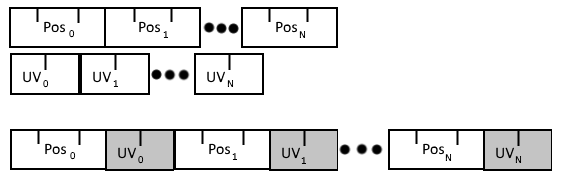
\includegraphics[width=\textwidth]{Main/Images/VertexInputLayoutVariants}
        %   \centering
        %   \caption{Layout of vertex input data when stored separately in multiple buffers (top) and interleaved in a single buffer (bottom).}
        %   \label{fig:VertexInputLayoutVariants}
        % \end{figure}

      \subsubsection{Input Assembly State}
        The input-assembly state describes how the input data to the vertex shader is interpreted.
        The most important parameter to set is the primitive topology.
        This is where the \gls{gpu} is told what kind of primitives the input data represents.
        For the purposes of this chapter, the chosen primitive topology is \lstinline{TRIANGLE_LIST}\footnote{Full name: \lstinline{VK_PRIMITIVE_TOPOLOGY_TRIANGLE_LIST}} as shown in listing~\ref{lst:InputAssemblyStateSetup}.

        \lstinputlisting[
          label=lst:InputAssemblyStateSetup,
          caption={Input assembly state setup .},
          style=MyCppFloat,
          firstline=34,
          lastline=35,
          float
        ]
        {Main/Listings/GraphicsPipelineSetup.cpp}

      \subsubsection{Tessellation State}
        \todo[inline]{Just omit this state and subsubsection? It's ignored when creating the graphics pipeline.}
        This state is only useful for the tessellation shader stage.
        In this chapter, only the vertex and fragment shader stages are in use so this state is ignored.

      \subsubsection{Viewport State}
      \label{sss:ViewportState}
        The viewport state specifies how many viewports and scissors are active in a pipeline.
        Both the viewport and scissor define a non-rotated rectangular region within the framebuffer that will be written to by shaders.
        Rendering results that would usually write to the entire extent of the framebuffer will be scaled down and displaced to fit into the viewport and cropped to be inside the scissor.
        See figure~\ref{fig:ViewportScissorSample} for an illustration of this.
        In this chapter, only one of each is used that include the entire framebuffer, respectively.

        \begin{figure}
          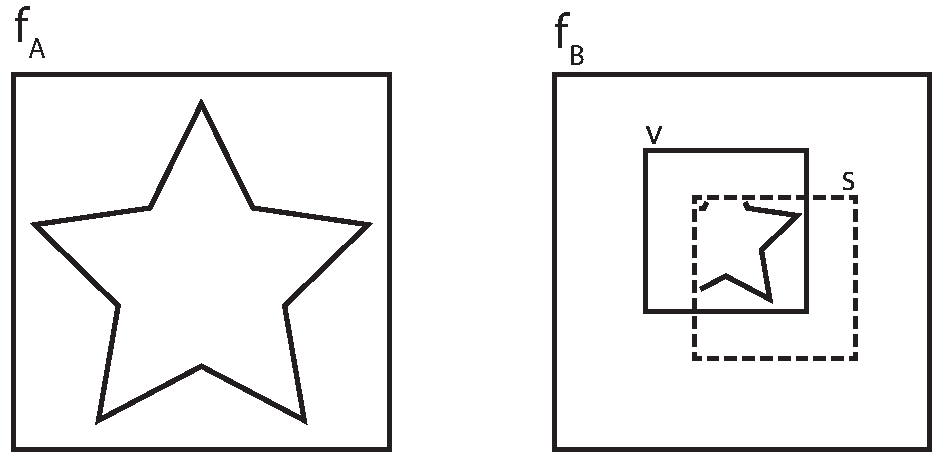
\includegraphics[width=0.666\textwidth]{Main/Images/ViewportScissorSample}
          \centering
          \caption{Framebuffer {\large$f_A$} has a viewport and scissor that contain the entire framebuffer. No transformation or cropping is performed. Framebuffer {\large$f_B$} has a viewport {\large$v$} that causes the contents to be displaced and scaled down as well as a scissor {\large$s$} that causes the remaining contents to be cropped.}
          \label{fig:ViewportScissorSample}
        \end{figure}

        There are two ways to specify the actual viewport and scissor data.
        The simplest way is to specify it at this point directly, i.e. when creating the graphics pipeline.
        However, this also means that the viewport and scissor data may never change during the lifetime of the pipeline.
        Changing the viewport and scissor data is necessary when the dimension of the render targets change.
        For example, when the application window is resized, the swapchain along with all swapchain images typically need to be re-created with dimensions matching the new window size, thus the viewport and scissor need to be updated as well.

        \lstinputlisting[
          label=lst:DynamicStateSetup,
          caption={Dynamic state setup for viewport and scissor state in chapter~\ref{cha:RenderPipeline}.},
          style=MyCppFloat,
          firstline=40,
          lastline=46,
          float
        ]
        {Main/Listings/GraphicsPipelineSetup.cpp}

        \lstinputlisting[
          label=lst:ViewportStateSetup,
          caption={Viewport state setup for chapter~\ref{cha:RenderPipeline}.},
          style=MyCppFloat,
          firstline=48,
          lastline=50,
          float
        ]
        {Main/Listings/GraphicsPipelineSetup.cpp}

        In order to prevent re-creating the entire graphics pipeline every time, which is a costly operation, the pipeline can be configured to accept \textit{dynamic state} as shown in listing~\ref{lst:DynamicStateSetup}.
        Dynamic state has to be set everytime when a render pass is being processed.
        Dynamic state data is recorded in command buffers and submitted along with the relevant render pass commands.

        Because dynamic state for the viewport and scissor data is used in this chapter, specifying the number of viewports and scissors as shown in listing~\ref{lst:ViewportStateSetup} is sufficient for the purpose of setting up a graphics pipeline.

      \subsubsection{Rasterization State}
        The rasterization state is used to configure the behavior of the rasterizer.
        It can be configured to control how fragments are produced and the circumstances in which they may be discarded.

        It is also used to control how primitves are rasterized.
        For example, given a triangle primitve, there are three ways for the rasterizer to produce fragments: Densely fill the entire rectangle, only produce fragments for the outline of the triangle, or just produce a fragment for each of the vertices, respectively.

        The rasterizer can also be configured to perform face culling, discarding fragments that are facing in a certain direction.
        Without this option, fragments are produced regardless of the direction they are facing.
        However, it is common to enable back-face culling which causes the rasterizer to discard fragments that would be viewed from ``behind''.
        In order to determine when a fragment is viewed from behind, the rasterizer needs to know the facing direction of a triangle\todo{Is it really just triangles? Use ``[...] facing direction of a (rendering) primitive'' instead?}.
        This facing direction is also configurable in the rasterizer state.
        It is defined by the winding order of the vertices, which is considered to be either \textit{clockwise} or \textit{counter-clockwise}.

        \lstinputlisting[
          label=lst:RasterizationStateSetup,
          caption={Rasterization state setup for chapter~\ref{cha:RenderPipeline}.},
          style=MyCppFloat,
          firstline=55,
          lastline=57,
          float
        ]
        {Main/Listings/GraphicsPipelineSetup.cpp}

        % \todo[inline]{I don't show a listing for any of the other pipeline states. This is an experiment to see how it would be if I backed the text with corresponding listings.}

        In listing~\ref{lst:RasterizationStateSetup}, the rasterizer is configured to produce densely filled polygons and does not perform any culling operations on the fragments.

      \subsubsection{Multisample State}
      \label{sss:MultisampleState}
        Multisampling is used to perform anti-aliasing, achieving a smoother appearance of jagged edges, and can be configured in the Multisample state.
        Disabling multisampling is not simply a matter of specifying the default value for all options.
        This state controls how many times the fragment shader is invoked and if a value of zero is passed as the number of samples, the fragment shader will never be invoked.

        \lstinputlisting[
          label=lst:MultisampleStateSetup,
          caption={Multisample state setup for chapter~\ref{cha:RenderPipeline}.},
          style=MyCppFloat,
          firstline=62,
          lastline=63,
          float
        ]
        {Main/Listings/GraphicsPipelineSetup.cpp}

        Multisampling is not being used in this chapter so the number of samples is set to one as shown in listing~\ref{lst:MultisampleStateSetup}.

      \subsubsection{Depth Stencil State}
        Depth and stencil tests are controlled in this state.
        Individual control is provided to enable depth testing, depth writing, depth bounds testing, as well as stencil testing.
        Depth bounds and comparison operations as well as stencil operations can be configured in this state.
        The comparison operation during depth tests can also be controlled.

        \lstinputlisting[
          label=lst:DepthStencilStateSetup,
          caption={Depth and stencil state setup for chapter~\ref{cha:RenderPipeline}.},
          style=MyCppFloat,
          firstline=68,
          lastline=72,
          float
        ]
        {Main/Listings/GraphicsPipelineSetup.cpp}

        In this chapter, stencil tests are disabled.
        Depth testing, on the other hand, is enabled with the typical less-or-equal comparison operation as shown in listing~\ref{lst:DepthStencilStateSetup}.

      \subsubsection{Color Blend State}
        The color blend state controls how color values produced by the fragment shader are combined, or blended, with the color that is already in the framebuffer.
        The blend operations need to be specified for each render target individually.
        \todo{Mention that a pipeline is needed for each material.}{}
        Blend operations may also be turned off which simply replaces whatever was in the framebuffer with the output of the fragment shader.

        In addition to controlling blending, a color mask can be set that controls which components of the resulting color values are written to the framebuffer.
        If a color mask of 0 is supplied, the framebuffer contents will remain unchanged.
        Likewise, a color mask with all bits set to 1 will copy all color components to the framebuffer.
        It is crucial to set this value correctly, otherwise undesired behavior may be observed.

        \lstinputlisting[
          label=lst:ColorBlendStateSetup,
          caption={Color blend state setup for chapter~\ref{cha:RenderPipeline}.},
          style=MyCppFloat,
          firstline=77,
          lastline=83,
          float
        ]
        {Main/Listings/GraphicsPipelineSetup.cpp}

        In this chapter, blending is turned off and a color mask is chosen so all color components are copied to the framebuffer as shown in listing~\ref{lst:ColorBlendStateSetup}.

        \todo[inline]{Give an example (transparent vs. non-transparent) if there is enough time.}

      \subsubsection{Render Pass}
      \label{sss:RenderPassSetup}
        In Vulkan, each graphics pipeline object is associated with a render pass.
        A render pass consists of multiple subpasses and stores information about the flow of data between subpasses and the execution of rendering commands.
        It stores framebuffer attachment and information about layout transitions at the beginning and the end of the render pass as well as between subpasses.
        Framebuffer attachments are images such as a swapchain image or a depth-buffer.
        Each of these subpasses may reference the aforementioned framebuffer attachments of the render pass.
        Dependencies of each subpass are also stored in the render pass.
        Rendering commands are always recorded to one of the subpasses of a render pass \textit{instance}.
        Command buffer recording is discussed in section~\ref{sec:BuildCommandBuffers}.

        \todo[inline]{Give an example about subpasses (post-processing) if there is enough time.}

        \lstinputlisting[
          label=lst:RenderPassAttachmentsSetup,
          caption={Setup of the attachments for the render pass used in chapter~\ref{cha:RenderPipeline}.},
          style=MyCppFloat,
          firstline=88,
          lastline=101,
          float
        ]
        {Main/Listings/GraphicsPipelineSetup.cpp}

        In listing~\ref{lst:RenderPassAttachmentsSetup}, the attachments for the render pass are being set up.
        The first attachment, attachment 0, is the render target which is actually a swapchain image.
        The format of that attachment is set to the same format as the surface.
        Like before in section~\ref{sss:MultisampleState}, the sampling count is set to 1, effectively disabling multisampling.
        On line~4, the render pass is configured to clear the contents of the first attachment at load-time.
        The value to clear the contents with is defined in the render pass instance.
        Once the render pass has finished executing, the \lstinline{storeOp} determines what happens to this attachment.
        In this case, on line~5, the framebuffer contents are preserved.
        Alternatively, the render pass can be configured to discard the results instead but that is not the desired behavior in this particular case.

        The subsequent settings are used to control the image layout at the beginning and the end of a render pass, respectively.
        On line~6, the initial layout of the attachment is specified to be undefined.
        This tells the \gls{driver} that it may discard the contents if it sees fit.
        The previous contents of the attachment are not relevant for this render pass because the attachment is cleared then loaded by this render pass.
        On line~7, the render pass is configured to ensure that the image layout state of the attachment is \lstinline{PRESENT_SRC}\footnote{Full name: \lstinline{VK_IMAGE_LAYOUT_PRESENT_SRC_KHR}}.
        This way no further transformations to the underlying swapchain image have to be performed before it can be presented.

        On lines 9--14, the depth buffer attachment is configured.
        The format of this attachment is set to the format of the actual depth buffer.
        Similarly to the first attachment, the depth buffer is cleared at the beginning of the render pass.
        The \lstinline{storeOp} is set to \lstinline{DONT_CARE}\footnote{Full name: \lstinline{VK_ATTACHMENT_STORE_OP_DONT_CARE}} because the depth buffer is not used outside the render pass.
        This is also the reason why both the initial and the final layout are simply set to \lstinline{DEPTH_STENCIL_ATTACHMENT}\footnote{Full name: \lstinline{VK_IMAGE_LAYOUT_DEPTH_STENCIL_ATTACHMENT_OPTIMAL}}.

        \lstinputlisting[
          label=lst:RenderPassSubpassSetup,
          caption={Setup of the single subpass for use in chapter~\ref{cha:RenderPipeline}.},
          style=MyCppFloat,
          firstline=103,
          lastline=115,
          float
        ]
        {Main/Listings/GraphicsPipelineSetup.cpp}

        As mentioned before, a render pass consists of multiple subpasses.
        Every render pass needs at least one subpass.
        For the purposes of this chapter, a single subpass is sufficient.
        This subpass is configured as shown in listing~\ref{lst:RenderPassSubpassSetup}.

        A subpass accepts configurations for the layout of individual attachments.
        Subpasses have references to the attachments of the render pass itself.
        These attachment references contain additional information, the most important one being the layout in that subpass.
        On line~2 of listing~\ref{lst:RenderPassSubpassSetup}, the index of the referenced attachment in the render pass is set.
        On line~3, the attachment reference is configured to ensure the correct image layout for the referenced attachment during the execution of that subpass.
        Every subpass within a render pass may define their own requirements for the layout of every individual attachment.
        Image layout transitions are performed by the \gls{driver} between subpasses as needed to ensure each subpass uses the attachment in the required layout.
        The depth-stencil reference on lines 6 and 7 is referencing the remaining attachment of the render pass and requires the \lstinline{DEPTH_STENCIL_ATTACHMENT} layout for this attachment.

        Note that the depth-stencil attachment reference on line~13 is only a single element, not an array.
        Color references on line~11 and 12, on the other hand, are not limited to a single instance.
        This means that a subpass may reference many color attachments but only a single depth-stencil attachment.

        \lstinputlisting[
          label=lst:RenderPassCreation,
          caption={Creation of a render pass object using the data defined in listings~\ref{lst:RenderPassAttachmentsSetup}~and~\ref{lst:RenderPassSubpassSetup}.},
          style=MyCppFloat,
          firstline=117,
          lastline=124,
          float,
          emph={RenderPass}
        ]
        {Main/Listings/GraphicsPipelineSetup.cpp}

        And finally, the attachment and subpass information defined previously are combined and passed to the appropriate Vulkan command on line~8 in listing~\ref{lst:RenderPassCreation} to create the actual render pass object.

    \subsection{Creating the Graphics Pipeline}
    \label{sub:ActualGraphicsPipelineCreation}
      In the previous section, the graphics pipeline was prepared to be created.
      Listing~\ref{lst:FinallyCreatingTheGraphicsPipeline} shows how all prepared data is combined in a single struct to finally produce a graphics pipeline object on line~16.

      \lstinputlisting[
        label=lst:FinallyCreatingTheGraphicsPipeline,
        caption={Combining all pipeline setup information to create a graphics pipeline object.},
        style=MyCppFloat,
        firstline=129,
        % lastline=101,
        float,
        emph={GraphicsPipeline}
      ]
      {Main/Listings/GraphicsPipelineSetup.cpp}

      The second parameter passed to \lstinline{vkCreateGraphicsPipelines} is the pipeline cache that was mentioned in section~\ref{subsec:PipelineCache}.
      In this case a \lstinline{VK_NULL_HANDLE} value is passed, thus no pipeline cache is used.
      If a valid pipeline cache object is passed, Vulkan would first check this cache for existing pipelines that match the input configuration.
      This is very likely to be faster than creating an entirely new pipeline.
      The exact algorithms and data structures used for managing pipeline caches are not defined by the Vulkan specification which means that \glspl{driver} are free to employ their own processing schemes.
      It should be noted that the pipeline cache is one of the rare cases where Vulkan guarantees internal synchronization, thus it is safe to use the same pipeline cache object across multiple threads.


    \subsection{Creating Framebuffers}
    \label{subsec:CreatingFramebuffers}
      A framebuffer defines the actual attachments that will be written to during a render pass.
      For the purposes of this chapter, each framebuffer references a swapchain image and a depth buffer image.
      Because there is usually more than one swapchain image, more than one framebuffer is required.
      Otherwise the framebuffer would need to be recreated every time a new swapchain image was acquired.
      A framebuffer also has dimensions that are defined when creating that framebuffer as shown below.
      These dimensions usually correspond to the dimensions of the referenced swapchain image.

      \lstinputlisting[
        label=lst:CreatingFramebuffers,
        caption={Creation of a set of framebuffers, one for each swapchain image.},
        style=MyCppFloat,
        float,
        emph={Framebuffers}
      ]
      {Main/Listings/CreatingFramebuffers.cpp}

      The process of creating the required framebuffers is shown in listing~\ref{lst:CreatingFramebuffers}.
      At first, a plain array of framebuffer handles is allocated using host memory.
      This array contains as many elements as there are swapchain images.
      Line~2 is the beginning of a loop that produces an index for every swapchain image with each iteration.
      On lines~4--6 the attachments of the framebuffer are defined.
      The first attachment is an image view to the swapchain image with the given index.
      The second attachment is the depth buffer that is the same for each framebuffer.
      It should be noted that the attachments are image \textit{views}, not plain images.
      Images are typically never used directly in Vulkan but rather referenced via image views that control which portion of the underlying image is used and how it is accessed.
      The image views used in this chapter all encompass the entirety of the images they reference.

      Following the attachment setup, the actual framebuffer info is constructed starting on line~8.
      It contains the attachments that were just specified, the render pass this framebuffer will be used for, the dimensions of the framebuffer in terms of a width, height, and layer count.
      Specifying the render pass at this point is not a hard restriction, it defines the types of render passes this framebuffer will be compatible with.
      And finally on line~15, a framebuffer is created and stored in the array created before.

    \subsection{Creating Scene Objects}
    \label{sss:CreatingSceneObjects}
      \todo[inline]{Mention push constants?}

      When creating scene objects, there are certain facilities that need to be set up on a per-object basis.
      In the example used throughout this chapter, every object needs to know how it can be translated from an application-specific space to clip space.
      Using this information, objects may be placed in different locations in the scene.
      The shader used for rendering them reflects this and is shown in section~\ref{sss:GraphicsPipelineShaderStages}.
      The descriptor set layout of the vertex shader, explained in section~\ref{sss:GraphicsPipelineLayout}, consists of only a single uniform buffer that contains information specific to an individual scene object.
      If a single instance of this information was shared among all scene objects, they would appear in the same location at once.
      Thus, a descriptor set, which adheres to the aforementioned descriptor set \textit{layout}, has to be created for each rendered object in the scene.

      The listings presented in this section are specific to each scene object.
      These listings may be thought of as depicting code inside of a loop that iterates all objects.

      \lstinputlisting[
        label=lst:AllocateUniformBuffer,
        caption={Allocation of a buffer object that will only be used as uniform buffer. Details about memory allocation are omitted.},
        style=MyCppFloat,
        firstline=1,
        lastline=9,
        float,
        emph={UniformBufferMemory, UniformBuffer}
      ]
      {Main/Listings/CreateSceneObjects.cpp}

      The first action to perform is to allocate a buffer for each object.
      This is shown in listing~\ref{lst:AllocateUniformBuffer}.
      When creating a buffer, Vulkan needs to know what the buffer will be used for.
      In this case the buffer will only be used as a uniform buffer object as specified on line~2.
      Details of allocating the memory for this buffer are omitted.
      However, for the purposes of this chapter, it is required that the memory is host-visible.
      Host-visible memory is needed in order to update the data without involving a separate command buffer that would upload and copy data on the device to the target buffer.
      This is important in the render loop discussed in section~\ref{sec:RenderLoop}.
      In order to make this buffer available during rendering, it needs to be bound to proper facilities because buffer objects do not provide information about where or how they are used in a shader.
      This information is provided by descriptor sets.
      Every descriptor set is tied to one or more descriptor set layouts.
      Only a single layout is used in this case which has been defined in section~\ref{sss:GraphicsPipelineLayout}.
      Descriptor sets can be bound to a command buffer to be used for a specific graphics pipeline, which is shown later when rendering commands are recorded in section~\ref{sec:BuildCommandBuffers}.

      \lstinputlisting[
        label=lst:DescriptorPoolCreation,
        caption={Creation of a descriptor pool which only supports allocating a single uniform buffer descriptor.},
        style=MyCppFloat,
        firstline=11,
        lastline=19,
        float,
        emph={DescriptorPool}
      ]
      {Main/Listings/CreateSceneObjects.cpp}

      \lstinputlisting[
        label=lst:DescriptorSetAllocation,
        caption={Allocation of a descriptor set.},
        style=MyCppFloat,
        firstline=21,
        lastline=26,
        float,
        emph={DescriptorSet}
      ]
      {Main/Listings/CreateSceneObjects.cpp}

      Descriptor sets are allocated from descriptor pools which also manage the underlying memory used by descriptor sets.
      The relationship between a descriptor pool and descriptor sets is similar to command pools and command buffers.
      Compared to command pools, however, descriptor pools are limited to a certain number of descriptor types that can be allocated from.
      These limits are defined by the application when a descriptor pool is created as shown in listing~\ref{lst:DescriptorPoolCreation}.
      On lines~2~and~3, the limit for uniform buffer descriptors is set to allow only a single allocation of that type.
      This limitation information is then used on line~8 to create the descriptor pool on line~9.
      The allocation of the descriptor set is shown in listing~\ref{lst:DescriptorSetAllocation}.
      Tying the descriptor set to a descriptor set layout is shown on line~4.

      \todo[inline]{Concluding sentence?}


  \section{Command Buffer Recording}
  \label{sec:BuildCommandBuffers}
    Rendering in Vulkan is done by issuing rendering commands.
    These commands are not dispatched to the \gls{gpu} directly but recorded into a \textit{command buffer} which is submitted to a device queue for execution.
    Submitted commands may be executed out-of-order, i.e. in a different order than they were recorded, if rearranging commands does not affect the resulting data.
    The \gls{driver} may do this in order to improve performance.
    This is analogous to how a compiler may rearrange instructions when performing optimizations to the code if this operation produces compatible results.
    Command buffers have been introduced in chapter~\ref{cha:VulkanOverview}, specifically section~\ref{sec:CommandBuffers}.

    \lstinputlisting[
      label=lst:CreateCommandBuffer,
      caption={Creation of a command pool and allocation of a command buffer.},
      style=MyCppFloat,
      firstline=1,
      lastline=9,
      float
    ]
    {Main/Listings/CreateCommandBuffer.cpp}

    Command buffer objects are created using \textit{command pools} as shown in listing~\ref{lst:CreateCommandBuffer}.
    Command pools manage the memory of the command buffers created from them.
    A command buffer is either in the \textit{initial}, \textit{recording}, or \textit{executable} state.
    The contents of a command buffer are immutable for as long as that command buffer is \textit{executable}.
    Resetting a command buffer clears its contents and reverts it to the \textit{initial} state.
    It must be noted that submitting a command buffer also does not clear its contents.
    This means that command buffers may be recorded once and executed multiple times.
    This can be very useful when recording a series of render commands for static scene geometry.
    It also improves performance insofar that the \gls{driver} is able to keep frequently used command buffers in \gls{gpu} memory, reducing required communication overhead between the \gls{cpu} and the \gls{gpu} and thus, reducing required bandwidth for data transmission.
    Rendering static scene geometry is a good example for these kinds of command buffers.
    This kind of geometry does not change over time, hence the commands required for rendering also do not change.

    For the purposes of this chapter, command buffers will only be recorded once and submitted in the render loop in section~\ref{sec:RenderLoop}.
    The framework defined before allows this to be possible because all objects in the scene are static in terms of rendering commands.
    However, this is only true because per-object shader data is stored in uniform buffer objects as established in section~\ref{sss:CreatingSceneObjects}.
    Uniform buffers are independent of the rendering commands and can be updated directly using memory mapping operations.
    Alternatively to uniform buffers, \textit{push constants} may be used to supply data to be used in shaders.
    Compared to uniform buffer objects, push constants have certain limitations that need to be considered.

    For each shader module, only a single \textit{push constant block} may be declared.
    The size of such a block is limited.
    The Vulkan specification requires that \glspl{driver} support sizes of at least 128 bytes but larger blocks may also be supported.
    The upper limit is specific to individual devices and can be queried using the Vulkan \gls{api}.
    Sizes of 256 bytes are common on current \gls{nvidia} hardware.
    Because of small sizes like this, push constants are likely to be stored in registers directly as opposed to uniform buffers which are stored in \gls{vram}.
    A note in section~13.2.6 also hints that using push constants may yield improved performance in terms of execution speed.

    The way values are supplied for push constant blocks is different from how a uniform buffer object is updated.
    Push constant values are updated using commands and are recorded to command buffers.
    This means that these values may be different for each recorded command buffer.
    If values are stored in the push constant block that changes every frame, such as the \gls{mvpmatrix} matrix of a scene object, command buffers need to be recorded every frame.

    \todo[inline]{Put a subsection here?}
    % \subsection{Rendering a Scene Object}
      % In this section, the necessary steps to record rendering commands for all scene objects are shown and explained.

      \lstinputlisting[
        label=lst:BeginCommandBuffer,
        caption={Start of the recording of a command buffer.},
        style=MyCppFloat,
        firstline=1,
        lastline=2,
        float
      ]
      {Main/Listings/CommandBufferRecording.cpp}

      % The first action that has to be performed is to start command buffer recording.
      Before issuing rendering commands, the command buffer has to be put into \textit{recording} state, which can be seen on line~2 of listing~\ref{lst:BeginCommandBuffer}.
      When beginning a command buffer, additional information can be passed in the \lstinline{VkCommandBufferBeginInfo} structure which can be seen on line~1.
      For example, this can be used to inform Vulkan that this particular command buffer is only submitted once which might allow the \gls{driver} to perform optimizations.
      For the purposes of this example, the default values are sufficient.

      \lstinputlisting[
        label=lst:DynamicStateUpdate,
        caption={Updating dynamic render pass state using Vulkan commands.},
        style=MyCppFloat,
        firstline=4,
        lastline=13,
        float
      ]
      {Main/Listings/CommandBufferRecording.cpp}

      Once the command buffer is \textit{recording}, the dynamic state can be set.
      As defined in section~\ref{sss:ViewportState}, the viewport and scissor data are part of the dynamic state.
      The commands for updating dynamic state are shown in listing~\ref{lst:DynamicStateUpdate}.
      The viewport is set to include the entire framebuffer on lines~2--3 as well as the entire depth buffer extent on lines~4--5.
      The scissor is set to contain the entire viewport on line~9, effectively disabling cropping of the resulting image.

      Dynamic state values are part of the command buffer.
      These values are read by graphics pipelines when executing draw commands without clearing them.
      This means that dynamic state only has to be set once for every command buffer if the values never change which is why dynamic state updates are the first commands recorded in the example of this chapter.
      These commands may be recorded at a later point if need be, but no later than before the first draw command is recorded.
      Additionally, setting these values is only necessary if the graphics pipeline has been set up to accept viewport and scissor data as dynamic state.
      Graphics pipelines that are not instructed to look for dynamic state will simply ignore the data in the command buffer and instead use the data supplied at pipeline creation.

      \lstinputlisting[
        label=lst:BeginRenderPass,
        caption={Creation of a render pass instance within a command buffer.},
        style=MyCppFloat,
        firstline=15,
        lastline=25,
        float,
        emph={vkCmdBeginRenderPass}
      ]
      {Main/Listings/CommandBufferRecording.cpp}

      In the next step, a render pass is started which results in the creation of a \textit{render pass instance} shown in listing~\ref{lst:BeginRenderPass}.
      This render pass instance is associated with a specific framebuffer on line~7 and clear values on line~10~and~11 that are used to clear attachment contents if their \lstinline{loadOp} is set to \lstinline{CLEAR}\footnote{Full name: \lstinline{VK_ATTACHMENT_LOAD_OP_CLEAR}}.
      The \lstinline{loadOp} settings were specified for each attachment in section~\ref{sss:RenderPassSetup}.
      Another property of the render pass instance is the render area on line~8.
      As can be seen, it is set to the same value as the scissor that was set before.
      The render area is used to control which pixels of the framebuffer are affected in the active render pass.
      This is used to minimize necessary work for the \gls{gpu}.
      A render area that is larger than the framebuffer is invalid.

      When beginning a render pass, Vulkan also needs to be told about whether secondary command buffers will be used or not.
      For the purposes of this chapter, only a single primary command buffer is used in a single subpass, which is why the render pass is instructed to inline render commands directly in the primary command buffer, disallowing execution of secondary command buffer.
      More information about command buffers was given in section~\ref{sec:CommandBuffers}.

      \lstinputlisting[
        label=lst:ObjectRenderingLoop,
        caption={Rendering of all scene objects.},
        style=MyCppFloat,
        firstline=27,
        lastline=40,
        float
      ]
      {Main/Listings/CommandBufferRecording.cpp}

      Now that a render pass instance is set up, draw commands can be recorded.
      Because there are multiple objects in the scene that need to be rendered, this will happen in a loop as can be seen on line~1 in listing~\ref{lst:ObjectRenderingLoop}.
      The first command causes the binding of a descriptor set with a specific pipeline layout.

      Afterwards, the command to bind the graphics pipeline is recorded on line~9.
      It is explicitly stated that the passed pipeline object is a graphics pipeline.

      With a pipeline in place, the vertex buffer and index buffer objects are bound.
      In both cases, the entire buffers are used, which is why all offsets are set to zero.
      As can be seen on line~11, multiple vertex buffers can be bound at once.
      Vertex buffers may be bound to different binding locations using the second argument to the depicted Vulkan API call, as long as these locations are valid for the given pipeline layout.
      In the case of this example, only a single vertex buffer is used per object that is bound to location 0.
      The indices in the index buffer contains unsigned 32~bit integer values.
      This information is passed to Vulkan on line~12.

      Following all the binding commands, the actual drawing command is issued.
      There are several drawing commands available but for the combination of objects that are bound only indexed drawing is valid.
      Because rendering is supposed to be done by using the bound index buffer, the drawing command to be recorded is \lstinline{vkCmdDrawIndexed}.
      The arguments are, in order, the number of indices to read from the index buffer, the number of instances to render, the index of the index buffer to use, an offset that is added to each value in the index buffer before it is used to perform vertex lookups, and finally the ID of the first instance to draw.
      Because instanced rendering is not intended, the instance count is set to 1 and the ID of the first instance is set to 0.
      The index buffer is assumed to be set up to reference every vertex directly.
      This means that the entire index buffer can be used with both offsets set to 0 and the count set to the number of available indices in the index buffer.

      \lstinputlisting[
        label=lst:ConcludingCommandBufferRecording,
        caption={Completion of the render pass and command buffer recording.},
        style=MyCppFloat,
        firstline=42,
        lastline=43,
        float
      ]
      {Main/Listings/CommandBufferRecording.cpp}

      Once all commands have been recorded, the render pass and the command buffer may be ended.
      This is shown in listing~\ref{lst:ConcludingCommandBufferRecording}.
      This transitions the command buffer from \textit{recording} to \textit{executable} state.
      The function \lstinline{vkEndCommandBuffer}, as seen on line~2, returns a status code of type \lstinline{VkResult}.
      If an error occurred during command buffer recording, all subsequent \lstinline{vkCmd*} calls will be ignored and an error code will be return when the command buffer is ended.
      For example, the command buffer may run out of memory early on and signal this once recording has ended.

      The command buffer is now ready for submission to a queue and execution on the \gls{gpu}.
      This is covered in section~\ref{sec:RenderLoop}.

      In the process presented above, only a single command buffer was recorded.
      For small amounts of commands like in this case, it might be beneficial to allocate a command buffer for each framebuffer and perform the recording for each of them.
      This avoids re-recording of command buffers every time a new swapchain image is acquired.


  \section{Rendering Loop}
  \label{sec:RenderLoop}
    This section presents the necessary operations that need to be performed for each rendered frame.
    It is assumed that the application runs inside of a loop in this section, as can be seen in the presented listings.

    % \lstinputlisting[
    %   label=lst:RenderLoop_SemaphoreCreation,
    %   caption={Creation of two semaphores used in the render loop.},
    %   style=MyCppFloat,
    %   firstline=1,
    %   lastline=5,
    %   float
    % ]
    % {Main/Listings/RenderLoop.cpp}

    \lstinputlisting[
      label=lst:RenderLoop_ShaderDataUpload,
      caption={Creation of two semaphores used in the render loop.},
      style=MyCppFloat,
      firstline=7,
      lastline=19,
      float
    ]
    {Main/Listings/RenderLoop.cpp}

    As defined by the framework in section~\ref{sec:Framework}, camera data is not fixed and may change over time.
    Thus, camera data has to be updated at some point during the rendering loop.
    After the camera data is updated, the uniform buffers of each object in the scene have to be updated as well.
    Listing~\ref{lst:RenderLoop_ShaderDataUpload} shows the loop in which this is done.
    For each object, the \gls{mvpmatrix} matrix is computed.
    Afterwards, the buffer memory is mapped to an actual memory location in \gls{cpu} accessible \gls{ram}.
    The computed \gls{mvpmatrix} matrix is then copied to the mapped memory region on line~12.
    On line~13, the memory mapping is undone to allow the \gls{driver} to reuse the memory region.

    \lstinputlisting[
      label=lst:RenderLoop_AcquireNextImage,
      caption={Creation of two semaphores used in the render loop.},
      style=MyCppFloat,
      firstline=21,
      lastline=29,
      float
    ]
    {Main/Listings/RenderLoop.cpp}

    The following step is to acquire the next free image from the presentation engine to be used for rendering.
    The necessary function call is shown in listing~\ref{lst:RenderLoop_AcquireNextImage}.
    Because this function may potentially block for as long as no swapchain image is available, it accepts a timeout argument.
    In this case, the maximum value for an unsigned 32~bit integer is passed, effectively waiting as long as possible for the function to return.
    \todo[fancyline]{Show how semaphores are created? It's neither particularly relevant nor very interesting...}
    This function also accepts a semaphore as fourth argument.
    This semaphore is needed because the presentation engine might not be finished reading from the image yet.
    Once the presentation engine is done processing the image, the semaphore is signaled.

    \lstinputlisting[
      label=lst:RenderLoop_QueueSubmission,
      caption={Submission of a command buffer to the device queue for rendering. Several semaphore are installed to ensure proper synchronization between the host and the device.},
      style=MyCppFloat,
      firstline=32,
      lastline=45,
      float
    ]
    {Main/Listings/RenderLoop.cpp}

    The next task depends on the exact setup of the system.
    If command buffers were created, one for each framebuffer, then the one corresponding to the acquired image may directly be submitted.
    This is assumed in listing~\ref{lst:RenderLoop_QueueSubmission}.
    If, on the other hand, only a single command buffer was allocated, it needs to be re-recorded at this point.
    Ideally, the application has put everything that is described in section~\ref{sec:BuildCommandBuffers} into a function which could now be called.
    However, this means that the \gls{driver} has to evaluate and upload the command buffer all over again.
    That is why pre-recording command buffers per framebuffer might be beneficial.
    The best course of action may vary and is a matter of performance evaluations on a per-application and possibly even per-platform basis.

    The command buffer that is in \textit{executable} state is now submitted to the queue for execution in listing~\ref{lst:RenderLoop_QueueSubmission}.
    When submitted command buffers, a number of semaphores may be passed that are used to ensure proper synchronization between the device and the host.
    On line~7, a semaphore is supplied that will be waited in the stages specified on line~5.
    It is the same semaphore that was used when acquiring the current swapchain image.
    In this particular, case it is set up so that color attachment writes are only performed after the presentation engine no longer reads from the image, thus properly synchronizing read and write access to the image.
    The semaphore on line~9 will be signaled once submitted command buffers have finished execution.
    This semaphore is used when presenting the image, which is explained next.


    \lstinputlisting[
      label=lst:RenderLoop_QueuePresent,
      caption={Creation of two semaphores used in the render loop.},
      style=MyCppFloat,
      firstline=47,
      lastline=57,
      float
    ]
    {Main/Listings/RenderLoop.cpp}

    \todo{Mention that command buffers need to be re-recorded before this \textbf{if} push constants are used.}
    Once command buffers have been submitted, the image they produce is presented to the application window.
    This process is shown in listing~\ref{lst:RenderLoop_QueuePresent}.
    First, the swapchain to perform the presentation with is specified on line~5.
    On line~6, the index of the image to present is given.
    Afterwards, on line~8, a semaphore is supplied.
    This semaphore will be waited on by the presentation engine before performing any reads on the specified image.
    It is the same semaphore shown earlier that is signaled once the submitted command buffers finished execution.
    In other words, the presentation engine waits until the \gls{gpu} has finished writing to the image before reading from the image in order to present it.
    On line~9, the actual present call is performed.

    % \lstinputlisting[
    %   label=lst:RenderLoop_QueueWaitIdle,
    %   caption={Creation of two semaphores used in the render loop.},
    %   style=MyCppFloat,
    %   firstline=59,
    %   lastline=63,
    %   float
    % ]
    % {Main/Listings/RenderLoop.cpp}



  % \section{Window Resizing}
  %   \todo[inline]{Should I actually add this section? (Only if there's enough time.)}
  %   \tbd

  \section{Multi-threaded Rendering}
  \label{sec:MultithreadedRendering}
    As mentioned in chapter~\ref{cha:VulkanOverview}, Vulkan API calls are not synchronized implicitly by the \gls{driver} in order to facilitate multi-threaded processing.
    However, this does not mean that multi-threading on the \gls{cpu} has not been taken into account when Vulkan was designed.
    There are actually several ways of utilizing multiple threads for rendering with Vulkan.
    Creating resources and recording command buffers from multiple threads are explored in the following subsections.

    \subsection{Multi-threaded Command Buffer Recording}
      A naive approach to utilize multi-threading is to create several command buffers and assign them to multiple threads.
      These threads would then record commands to their assigned command buffers and submit them to a device queue.
      Unfortunately, there are some problems with this approach.
      According to sections~5.3~and~5.4 of the Vulkan specification~\cite{vkspec}, the host application is responsible for synchronizing interactions with command buffers and submitting them to device queues.

      % Problem with command buffers and multi-threaded access.
      Command buffer access is not thread-safe.
      This is because memory used by command buffers is managed by the parent command pool.
      The actual algorithms used for managing memory are left to the \gls{driver}.
      % Done for implementations to be more memory efficient.
      This allows command pools efficient handling of memory operations performed by multiple command buffers, e.g. by allocating more memory than is currently needed and reassigning it as more is requested.
      % Command buffers work on memory managed by parent command pool.
      Because command pools are free to manage memory as they see fit, any operation on a command buffer may trigger side-effects that affect other command buffers created from the same pool.
      This fact alone makes command buffers unsuitable to be shared across multiple threads without synchronization.

      % Command pools do not depend on anything else.
      Command pools, on the other hand, are independent objects.
      The memory they manage is only used for command buffers they created.
      Whenever available memory is no longer sufficient, new memory from the host is requested, optionally using a application-supplied allocator.
      This allocator needs to synchronize low-level allocations, like the C standard library function \lstinline{malloc} already does.
      % Thus solution is to assign each thread its own command pool.
      Synchronization of low-level memory allocation is certainly not as costly as synchronizing each command buffer access.
      Typically, those low-level memory allocations do not happen very often.
      It is likely that command pool implementations strive for minimal host allocations.

      Command pools effectively do not need to be manually synchronized across multiple threads if they are not shared between them.
      In addition, command buffers created from such command pools inherit the same properties.
      Thus, it is more suitable to assign one or more command pools per thread.
      % Threads then allocate and record into as many command buffers as needed.
      Each thread is then free to allocate and record into as many command buffers as needed without having to conduct fine-grained synchronization.

      % Let main thread submit command buffers by sharing a datastructure with synchronized access.
      In order for command buffers allocated on other threads to be submitted to the device queue, the main thread may provide a shared datastructure that is capable of containing command buffer objects.
      Access to this shared container would be synchronized using traditional synchronization methods.
      % Turns the initial problem into well-understood producer-consumer problem~\cite{EWD:EWD329}.
      % Solves the inital queue submission problem.
      This effectively creates the well-understood producer-consumer scenario~\cite{EWD:EWD329} and solves the initial queue submission problem.

      \todo[inline]{Prev paragraph is just a suggestion. May be better to do differently. Depends on application.}

      \subsubsection{Command Buffer Management Considerations}
        % ... There is another problem with the system mentioned above.
        % ... It is also recommended to assign more than one command pool to an individual thread.
        % ... While a command buffer is being processed, i.e. once it has been submitted but has not finished execution yet, the command buffer should not be modified.
        % ... The reason why multiple pools should be used instead of simply creating new command buffers from the same pool is because of the underlying memory model.

        % ... In the previously described scenario, each thread has exactly one command pool that is used to create multiple command buffers from.
        % ... Commands are recorded to these command buffers and are submitted in batches to the device for execution.
        % ... Vulkan specifies some restrictions on what may be done with command buffers that are pending execution.
        % ... For example, the application should not free a command buffer that is pending execution.

        % Command buffers need to be kept alive while pending execution.
        Vulkan prohibits modifying submitted command buffers that are pending execution on the device.
        This includes freeing these command buffers which implies that the application is responsible for keeping them alive as long as they are pending execution.
        In practice, this effectively means command buffers submitted in batches may only be modified or reused once the entire submission has finished execution because it is hard to predict when individual commands are processed if more than one command buffer is submitted.
        Out-of-order execution is one reason for this unpredictability.
        An application could insert events to track completion of individual command buffers, but this would impose additional synchronization overhead on the \gls{gpu}.
        Additionally, if all allocated command buffers are still in use, and new commands need to be recorded, the application either has to wait for a command buffer to finish or dynamically allocate new command buffers from a pool.
        The simplest way to solve this problem is to always use new command buffers for every new batch submission.
        The host application would need to track these command buffers somehow in order to be freed or reused.
        Vulkan does not do this automatically.
        Otherwise, if command buffers are never freed, the application ends up allocating a lot more than necessary, effectively leaking memory.

        % Command pools better than just using command buffers because of decoupled underlying memory and clean separation of concern.
        A better way might be to use command pools for this purpose.
        Managing command buffers is already what they do and it also offers a clean separation of concerns between the different batches of command buffers.
        In other words, using command pools to allocate command buffers that are submitted together provides a way to manage these command buffers using standard methods.
        Vulkan allows command pools to be reset, effectively resetting all command buffers spawned from them.
        This means that command pools may be reused after their associated batch of submitted command buffers has finished execution.
        When resetting a command pool, the host application is free to choose whether memory allocated by that command pool should be released or not.
        If a command pool is going to be reused, and the memory is not released, this command pool can directly start producing command buffers without causing additional allocation overhead.
        This provides a clean way for managing command buffer lifetimes without the need to use anything but the Vulkan \gls{api} itself.

        \todo{Describe what they did differently?}Similar approaches have been described by industry experts such as Marius Bjørge~\cite{bjorge:multithreadingvulkan} in his blog post about multi-threading in Vulkan as well as Mathias Schott~\cite{mschott:vulkan_multi_threading} in his talk entitled ``Vulkan multi-threading''.

        Care must be taken, however, in cases where the amount of memory required by a command buffer is not steady during its lifetime.
        For example, when transitioning from a large \gls{3d} scene, with many objects to render, to a small scene with less draw calls to perform, the memory requirements of each command buffer may be lowered considerably for the new scene.
        In cases like this, it might make sense to reset all relevant command buffers, freeing their associated memory.
        Switching from a small scene to larger one is not a problem, of course, because the command buffer will simply allocate enough memory for the new scene.


    \subsection{Multi-threaded Resource Creation}
      \todo[inline]{Mention staging buffers somehow?}
      Vulkan applications need to create resources such as images and shaders.
      Loading and creating these resources may take a considerable amount of time, depending on the data in question.
      Images, for example, can be quite large.
      They may also have to be transformed in some way which also consumes computation time.
      Shaders need to be compiled (by the \gls{driver}) and bound to a Vulkan pipeline.
      Many of these time consuming operations work more or less independently from the rest of the system, depending on the specific operation.
      This makes them interesting candidates for execution on multiple threads.
      However, the use of multi-threaded resource creation introduces additional complexity to the system.

      First of all, an application has to decide how many threads are actually needed for resource creation.
      It is possible that only one dedicated resource creation thread is sufficient for many applications.
      The actual number of resource creation threads depends on the application.

      All resource creation threads need device memory in one way or another.
      There are basically two ways of accomplishing this without race conditions.
      The first way is to preallocate the memory that is available for each thread.
      This method does not require synchronization between threads because each is assigned a memory region that is not overlapping memory from other threads.
      The second way is to assign a memory allocator to each thread that internally synchronizes the calls.
      This method does not require the main thread to know the size of the resources each thread creates but memory allocations need to be synchronized.
      Again, the method of choice depends on the application.
